% Current BCS model (v2), "Attention Is All You Need" style (bottom-to-top flow).
% Left: region segmenter (DINOv2-B fine-tuned + FPN, 40 annotated + 345 pseudo-labeled frames).
% Right: frozen DINOv3-L/16 at 384 px, output of block 21 of 24 -> per-region average -> ridge -> BCS.
% v1 (DINOv2-L, last block) is in model_bcs.tex.
% Build: pdflatex model_bcs_v2.tex
\documentclass[tikz,border=8pt]{standalone}
\usepackage[utf8]{inputenc}
\usepackage[T1]{fontenc}
\usetikzlibrary{arrows.meta,calc,backgrounds,fit}

\definecolor{attn}{HTML}{FCE0C4}
\definecolor{norm}{HTML}{F3F5C9}
\definecolor{ff}{HTML}{C9E7F5}
\definecolor{emb}{HTML}{FADADD}
\definecolor{dec}{HTML}{DCD3EE}
\definecolor{reg}{HTML}{D5EBD9}
\definecolor{bloque}{HTML}{F2F2F2}
\definecolor{nota}{HTML}{666666}

\tikzset{
  font=\sffamily\small, >={Stealth[length=2mm]},
  capa/.style={draw, rounded corners=4pt, line width=0.6pt, minimum width=3.4cm,
               minimum height=0.62cm, align=center, fill=#1},
  alta/.style={capa=#1, minimum height=0.95cm},
  suma/.style={draw, circle, line width=0.6pt, inner sep=0pt, minimum size=0.42cm, fill=white},
  flecha/.style={->, line width=0.6pt},
  linea/.style={line width=0.6pt},
  marco/.style={draw, rounded corners=8pt, line width=0.6pt, fill=bloque},
  ls/.style={draw, rounded corners=3pt, line width=0.6pt, minimum width=2.0cm, minimum height=0.4cm, fill=white, font=\sffamily\scriptsize},
  lado/.style={font=\sffamily\scriptsize, text=nota, align=left},
}
\newcommand{\plus}[2]{\node[suma] (#1) at #2 {};
  \draw[line width=0.6pt] (#1.north) -- (#1.south) (#1.west) -- (#1.east);}

% Transformer encoder block (pre-norm) centered at x=#1, name prefix #2, attention label #3
\newcommand{\bloque}[3]{
  \draw[linea] (#1,2.15) -- (#1,2.95);
  \node[capa=norm] (#2ln1) at (#1,3.55) {Layer Norm};
  \node[alta=attn] (#2mha) at (#1,4.85) {#3};
  \node[ls]        (#2ls1) at (#1,5.8) {LayerScale};
  \plus{#2add1}{(#1,6.4)}
  \node[capa=norm] (#2ln2) at (#1,7.25) {Layer Norm};
  \node[alta=ff]   (#2mlp) at (#1,8.45) {MLP};
  \node[ls]        (#2ls2) at (#1,9.4) {LayerScale};
  \plus{#2add2}{(#1,10.0)}
  \draw[flecha] (#1,2.95) -- (#2ln1);
  \draw[linea] (#2ln1.north) -- ++(0,0.2) coordinate (#2qkv);
  \foreach \dx in {-0.8,0,0.8} \draw[flecha] (#2qkv) -| ($(#2mha.south)+(\dx,0)$);
  \draw[flecha] (#2mha) -- (#2ls1); \draw[flecha] (#2ls1) -- (#2add1); \draw[flecha] (#2add1) -- (#2ln2);
  \draw[flecha] (#2ln2) -- (#2mlp);  \draw[flecha] (#2mlp) -- (#2ls2); \draw[flecha] (#2ls2) -- (#2add2);
  \draw[flecha, rounded corners=3pt] (#1,3.05) -- ++(-2.15,0) |- (#2add1.west);
  \draw[flecha, rounded corners=3pt] (#1,6.8) -- ++(-2.15,0) |- (#2add2.west);
  \begin{scope}[on background layer]
    \node[marco, fit={(#1-2.35,2.8) (#1+1.95,10.4)}] (#2blk) {};
  \end{scope}
}

\begin{document}
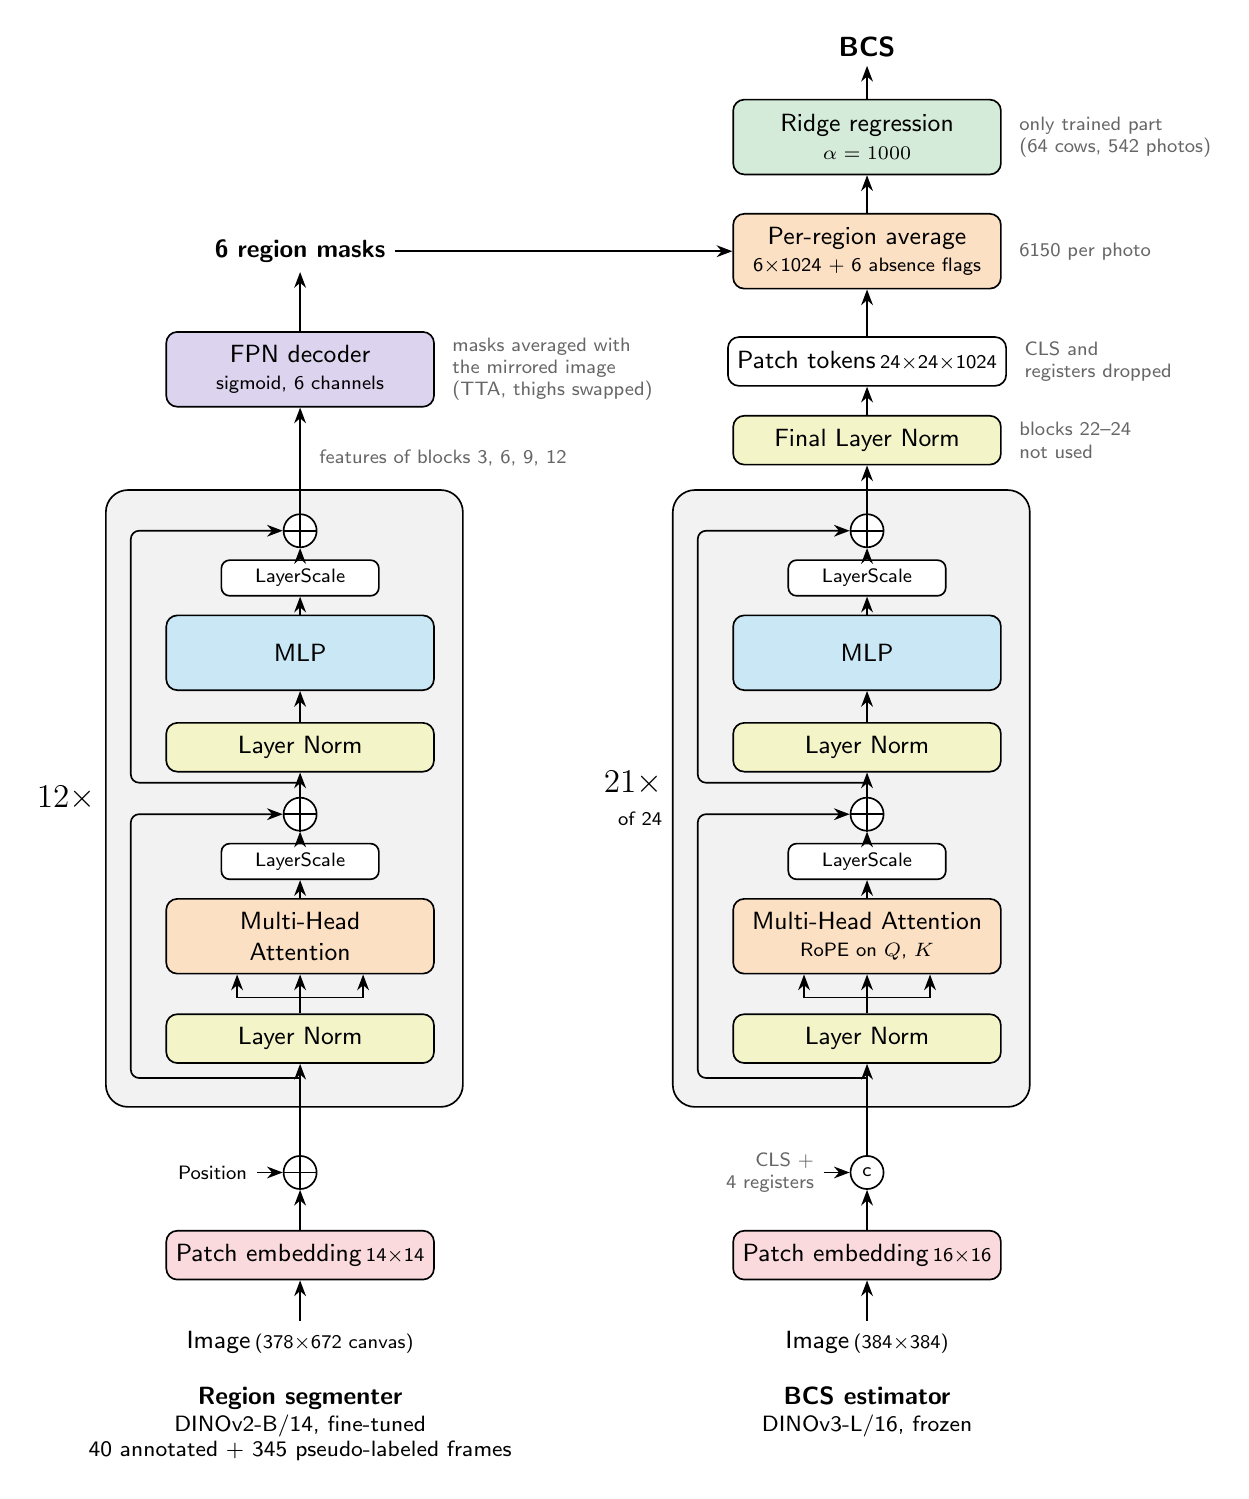
\begin{tikzpicture}

% ---------- Region segmenter: DINOv2-B (learned absolute position) ----------
\node (Ain) at (0,-0.3) {Image\,\scriptsize(378$\times$672 canvas)};
\node[capa=emb] (Ape) at (0,0.8) {Patch embedding\,\scriptsize14$\times$14};
\plus{Apos}{(0,1.85)}
\node[anchor=east, font=\sffamily\scriptsize] (Apost) at (-0.55,1.85) {Position};
\draw[flecha] (Ain) -- (Ape); \draw[flecha] (Ape) -- (Apos); \draw[flecha] (Apost) -- (Apos);
\draw[linea] (Apos.north) -- (0,2.15);
\bloque{0}{A}{Multi-Head\\Attention}
\node[font=\sffamily\large, anchor=east] at (Ablk.west) {$12\times$};
\node[alta=dec] (fpn) at (0,12.05) {FPN decoder\\[-1pt]\scriptsize sigmoid, 6 channels};
\node (masks)         at (0,13.55) {\textbf{6 region masks}};
\draw[flecha] (Aadd2) -- (fpn);
\node[lado, anchor=west] at (0.12,10.92) {features of blocks 3, 6, 9, 12};
\node[lado, anchor=west] at ($(fpn.east)+(0.1,0)$) {masks averaged with\\the mirrored image\\(TTA, thighs swapped)};
\draw[flecha] (fpn) -- (masks);
\node[font=\sffamily\small\bfseries, align=center, anchor=north] at (0,-0.75)
  {Region segmenter\\[-1pt]\mdseries\footnotesize DINOv2-B/14, fine-tuned\\[-2pt]\mdseries\footnotesize 40 annotated + 345 pseudo-labeled frames};

% ---------- BCS estimator: DINOv3-L/16 (RoPE, register tokens), frozen ----------
\def\xb{7.2}
\node (Bin) at (\xb,-0.3) {Image\,\scriptsize(384$\times$384)};
\node[capa=emb] (Bpe) at (\xb,0.8) {Patch embedding\,\scriptsize16$\times$16};
\node[draw, circle, line width=0.6pt, inner sep=0pt, minimum size=0.42cm, fill=white, font=\sffamily\scriptsize] (Bcat) at (\xb,1.85) {c};
\node[anchor=east, lado, align=right] (Bpre) at (\xb-0.55,1.85) {CLS +\\4 registers};
\draw[flecha] (Bin) -- (Bpe); \draw[flecha] (Bpe) -- (Bcat); \draw[flecha] (Bpre) -- (Bcat);
\draw[linea] (Bcat.north) -- (\xb,2.15);
\bloque{\xb}{B}{Multi-Head Attention\\[-1pt]\scriptsize RoPE on $Q$, $K$}
\node[font=\sffamily\large, anchor=east, align=right] at (Bblk.west) {$21\times$\\[-2pt]\scriptsize of 24};
\node[capa=norm]  (fnorm) at (\xb,11.15) {Final Layer Norm};
\node[capa=white] (tok)   at (\xb,12.15) {Patch tokens\,\scriptsize24$\times$24$\times$1024};
\node[alta=attn]  (pool)  at (\xb,13.55) {Per-region average\\[-1pt]\scriptsize 6$\times$1024 + 6 absence flags};
\node[alta=reg]   (ridge) at (\xb,15.0)  {Ridge regression\\[-1pt]\scriptsize $\alpha = 1000$};
\node[font=\sffamily\bfseries] (bcs) at (\xb,16.15) {BCS};
\draw[flecha] (Badd2) -- (fnorm); \draw[flecha] (fnorm) -- (tok); \draw[flecha] (tok) -- (pool);
\draw[flecha] (pool) -- (ridge); \draw[flecha] (ridge) -- (bcs);
\draw[flecha] (masks) -- (pool);
\node[lado, anchor=west] at ($(tok.east)+(0.1,0)$) {CLS and\\registers dropped};
\node[lado, anchor=west] at ($(fnorm.east)+(0.1,0)$) {blocks 22--24\\not used};
\node[lado, anchor=west] at ($(pool.east)+(0.1,0)$) {6150 per photo};
\node[lado, anchor=west] at ($(ridge.east)+(0.1,0)$) {only trained part\\(64 cows, 542 photos)};
\node[font=\sffamily\small\bfseries, align=center, anchor=north] at (\xb,-0.75)
  {BCS estimator\\[-1pt]\mdseries\footnotesize DINOv3-L/16, frozen\\[-2pt]\mdseries\footnotesize\phantom{p}};

\end{tikzpicture}
\end{document}
